We plot the melspectrogram of raw speech, resynthesized speech of EnCodec RVQ-1 tokens, and resynthesized speech of \method RVQ-1 tokens. From the figure~\ref{fig:mel}, it's evident that the melspectrogram corresponding to EnCodec RVQ-1 largely retains the stripes and shapes in the raw melspectrogram. In contrast, the speech resynthesized from \method RVQ-1 essentially loses all of the horizontal stripes, which indicates that timbre and prosody information has been diminished.

\begin{figure*}[h] 
    % \vspace{-5pt}
    \centering 
    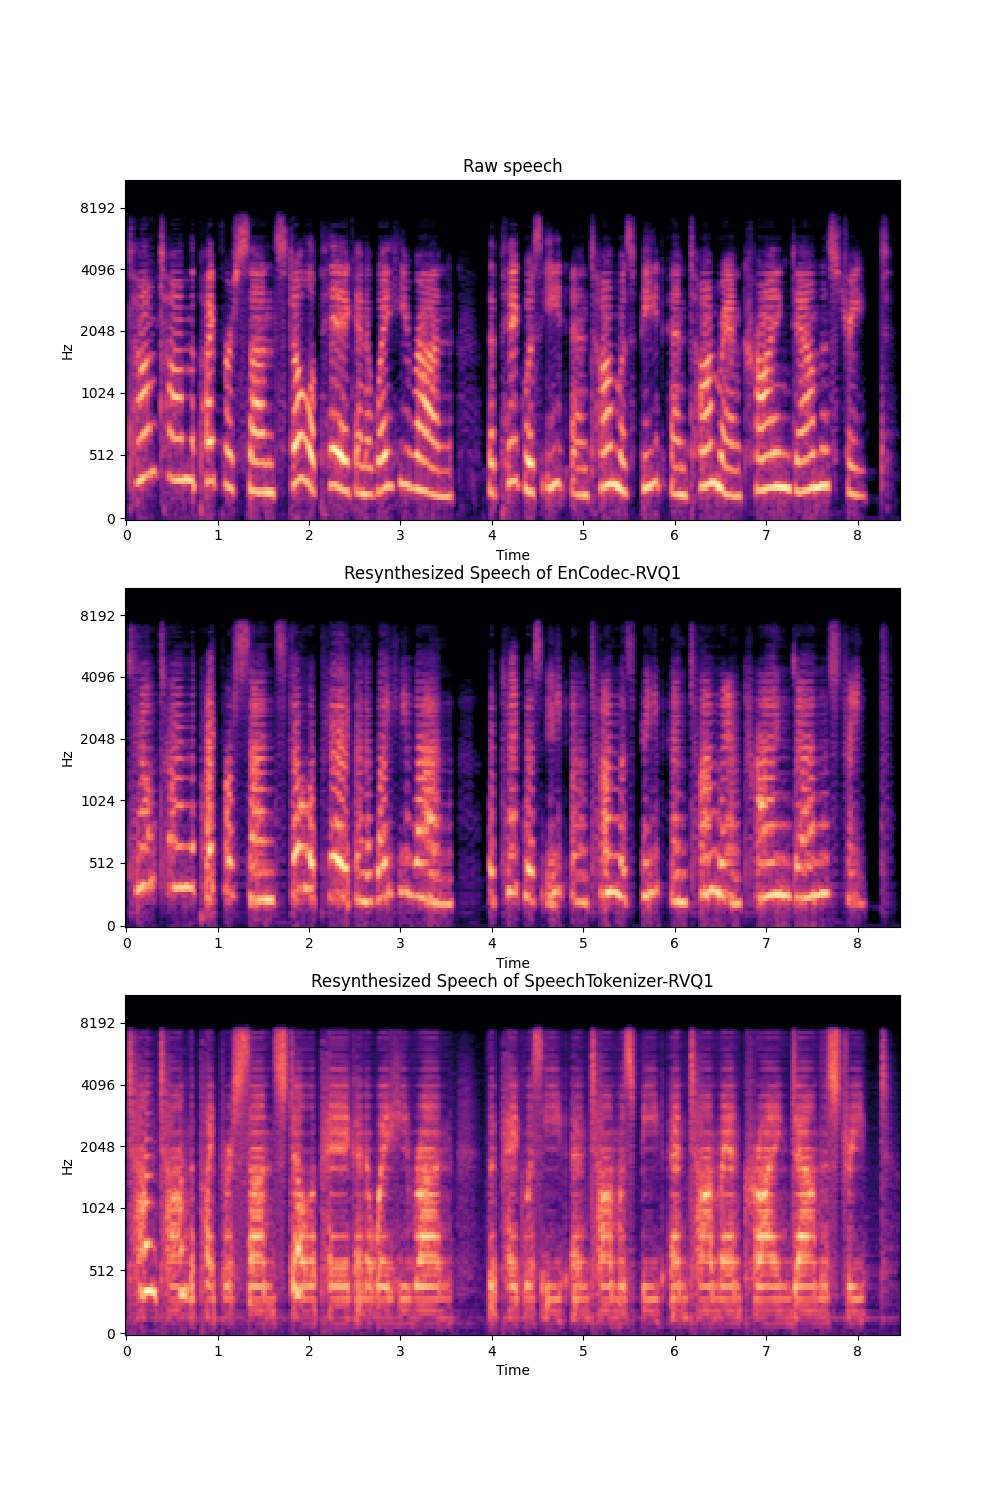
\includegraphics[width=0.8\textwidth]{Figures/mel.png} 
    \caption{Melspectorgram of raw speech, resynthesized speech of \method and EnCodec RVQ-1 tokens.}

    \label{fig:mel} 
\end{figure*}

\clearpage

We alse plot melspectrogram of raw German speech and resynthesized German speech of \method RVQ-1 tokens. 
As shown in the Figure~\ref{fig:mel_de}, the same patterns observed in English speech are also present in German speech.



\begin{figure*}[h] 
    % \vspace{-5pt}
    \centering 
    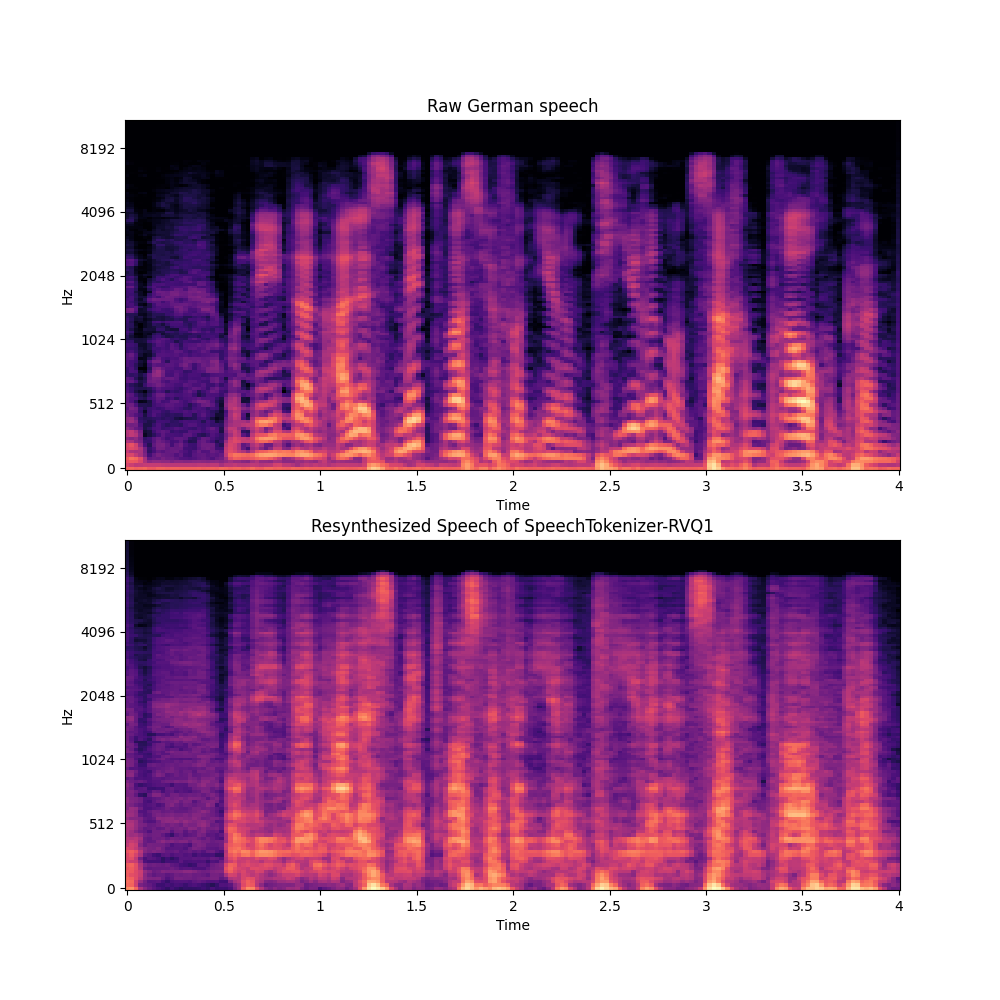
\includegraphics[width=0.8\textwidth]{Figures/mel_de.png} 
    \caption{Melspectorgram of German speech and resynthesized speech of \method RVQ-1 tokens.}

    \label{fig:mel_de} 
\end{figure*}